\documentclass[a4paper, 12pt]{article}
\usepackage[utf8]{inputenc}
\usepackage[russian,english]{babel}
\usepackage[T2A]{fontenc}
\usepackage[left=10mm, top=20mm, right=10mm, bottom=15mm, footskip=13mm]{geometry}
\usepackage{indentfirst}
\usepackage{amsmath,amssymb}
\usepackage{graphicx}
\usepackage[italicdiff]{physics}
\usepackage{float}
\usepackage{array}
\usepackage{physics}
\graphicspath{ {shema/} {graphic/} }
\usepackage{caption}
\captionsetup[figure]{name=Рисунок}
  
\title{Отчет по лабораторной работе 1.1.6

ИЗУЧЕНИЕ ОСЦИЛЛОГРАФА}

\author{Максим Осипов, Б03-504}
\date{15.10.2025}

\begin{document}
\maketitle
\newpage
\section{Аннотация}
Цель работы: ознакомиться с устройством и органами управления
электронного и/или цифрового осциллографа; научиться измерять амплитуды и частоты произвольных сигналов; изучить основные характеристики осциллографа и их влияние на искажение сигналов.\\

\hspace{0,01cm}В работе используются: осциллограф (электронный и/или цифровой), генераторы электрических сигналов, соединительные кабели.

\section{Теоретическая справка}


\subsection*{Устройство и принцип работы осциллографа}

\textbf{Осциллограф} -- регистрирующий прибор, в котором исследуемый электрический сигнал преобразуется в видимый на экране график изменения величины сигнала во времени.

\subsection*{Электронно-лучевая трубка}

Основные элементы ЭЛТ:
\begin{itemize}
\item[1.] Подогреватель катода
\item[2.] Катод
\item[3.] Модулятор (управление яркостью)
\item[4.] Фокусирующий анод
\item[5.] Ускоряющий анод
\item[6,7.] Отклоняющие пластины (горизонтальные и вертикальные)
\item[8.] Ускоряющий анод
\item[9.] Экран 
\end{itemize}

\begin{figure}[h]
\centering
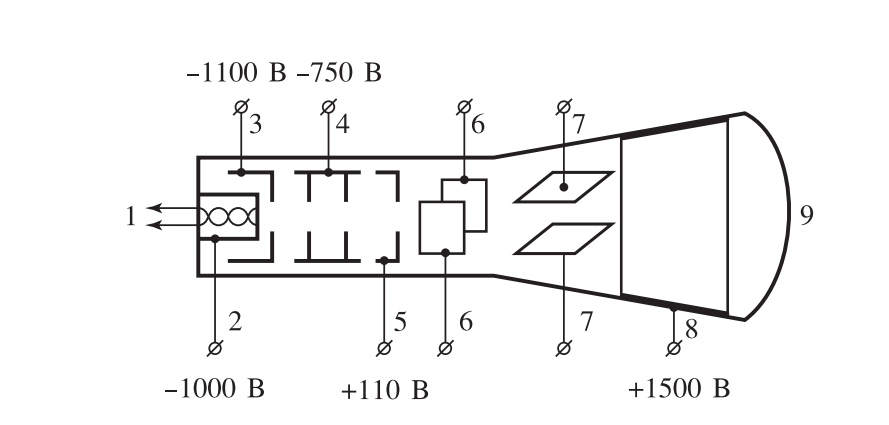
\includegraphics[width=0.8\linewidth]{рис 1.png}
\caption{Электронно-лучевая трубка}
\label{fig:voltage_current}
\end{figure}

\subsection*{Движение электронов в поле отклоняющих пластин}

Траектория электрона между пластинами:
\begin{equation}
y = \frac{eU_y}{2mv_0^2}z^2
\end{equation}

Смещение пучка и угол отклонения:
\begin{equation}
y_1 = \frac{eE_y}{2mv_0^2}l^2, \quad \tg\alpha = \frac{eE_y}{mv_0^2}l
\end{equation}

Полное смещение на экране:
\begin{equation}
h = y_1 + L\tg\alpha = \frac{e(l/2 + L)}{2mv_0^2}E_y
\end{equation}

Связь скорости электронов с ускоряющим напряжением:
\begin{equation}
\frac{mv_0^2}{2} = eU_a
\end{equation}

Окончательное выражение для смещения:
\begin{equation}
h_y = \frac{l(l/2 + L)}{2dU_a} \cdot U_y
\end{equation}

Чувствительность трубки:
\begin{equation}
K_y = \frac{U_y}{h} = \frac{2dU_a}{l(l/2 + L)} \quad \text{[В/см]}
\end{equation}

\begin{figure}[h]
\centering
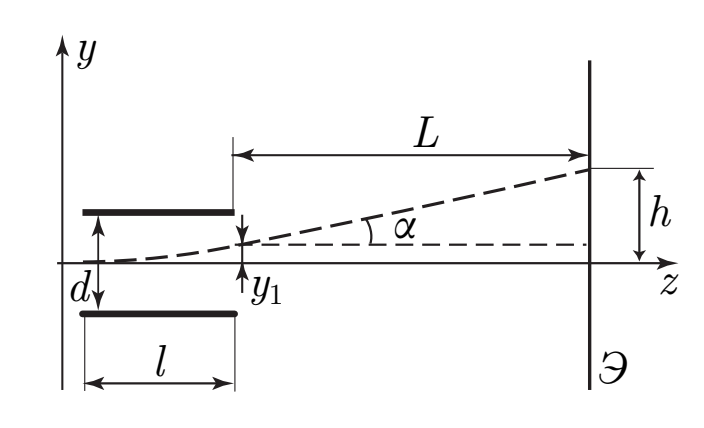
\includegraphics[width=0.8\linewidth]{рис 2.png}
\caption{Отклонение луча в электрическом поле пластин}
\label{fig:voltage_current}
\end{figure}

\subsection*{Полоса пропускания}

Формула (5) применима при условии $T \gg \tau$, где $\tau = l/v_0$ -- время пролёта между пластинами. При $U_a = 2$ кВ, $v_0 \sim 3\cdot10^7$ м/с, $l = 3$ см получаем $\tau \sim 10^{-9}$ с.

\subsection*{Режимы работы}

\textbf{Развёртка:}
\begin{equation}
U_y(t) = U_{0y} + K_yU(t), \quad U_x = U_{0x} + kt
\end{equation}

\textbf{Входные режимы:}
\begin{itemize}
\item Закрытый вход (AC) -- только переменная составляющая
\item Открытый вход (DC) -- постоянная и переменная составляющие
\end{itemize}

\begin{figure}[h]
\centering
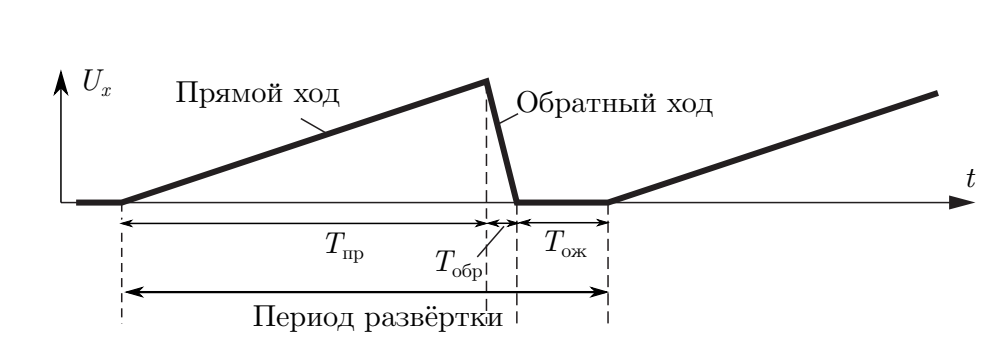
\includegraphics[width=0.8\linewidth]{рис 3.png}
\caption{Напряжение развёртки}
\label{fig:voltage_current}
\end{figure}

\begin{figure}[h]
\centering
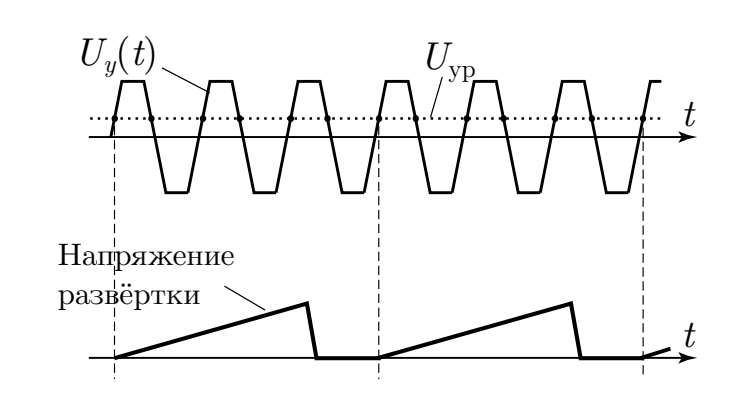
\includegraphics[width=0.75\linewidth]{рис 4.png}
\caption{Синхронизация развёртки по заданному уровню (по нарастанию)
}
\label{fig:voltage_current}
\end{figure}

\subsection*{Амплитудно-частотная и фазо-частотная характеристики}

Для гармонического сигнала $U_y = U_0\sin 2\pi\nu t$ на экране:
\begin{equation}
y = y_0\sin(2\pi\nu t + \phi)
\end{equation}

АЧХ:
\begin{equation}
K(\nu) = \frac{y_0(\nu)}{U_0}
\end{equation}

Полоса пропускания определяется по уровню:
\begin{equation}
\frac{K(\nu_{min})}{K_{max}} = \frac{K(\nu_{max})}{K_{max}} = \frac{1}{\sqrt{2}} \approx 0,7
\end{equation}

\subsection*{Фигуры Лиссажу}

При подаче сигналов:
\begin{equation}
U_y(t) = U_{0y}\sin(2\pi\nu_yt + \phi_y), \quad U_x(t) = U_{0x}\sin(2\pi\nu_xt + \phi_x)
\end{equation}

Для колебаний одинаковой частоты:
\begin{equation}
x = A\cos(2\pi\nu t + \phi_x), \quad y = B\cos(2\pi\nu t + \phi_y)
\end{equation}

Уравнение траектории:
\begin{equation}
\frac{x^2}{A^2} + \frac{y^2}{B^2} - 2\frac{xy}{AB}\cos\Delta\phi = \sin^2\Delta\phi
\end{equation}
где $\Delta\phi = \phi_y - \phi_x$.

Отношение частот определяется по числу пересечений:
\begin{equation}
\frac{\nu_y}{\nu_x} = \frac{n_x}{n_y}
\end{equation}

\begin{figure}[h]
\centering
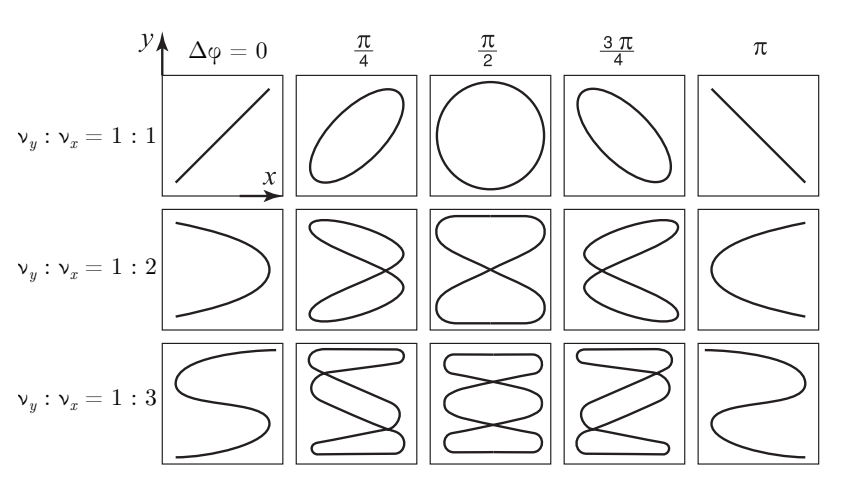
\includegraphics[width=0.8\linewidth]{рис 5.png}
\caption{Фигуры Лиссажу (для колебаний одинаковой амплитуды)
}
\label{fig:voltage_current}
\end{figure}


\end{document}
